% preambula dokumenta
\documentclass[a4paper, 10pt]{article}
\usepackage[slovene]{babel}
\usepackage[utf8]{inputenc}
\usepackage[T1]{fontenc}
\usepackage{lmodern}
\usepackage[pdftex]{graphics}
\usepackage{amsmath}
\usepackage{graphicx}
\usepackage{eurosym}
\usepackage{float}
\graphicspath{ {./images/} }

\renewcommand*\contentsname{Kazalo}
\pagenumbering{arabic}

% telo dokumenta
\begin{document}

\begin{titlepage}
\begin{center}

\Huge 
\textbf{Predpostavka o Randićevem indeksu in radiusu}

\vspace{1cm}
\Large
\textbf{Poročilo pri predmetu Finančni praktikum}

\vspace{1cm}

\vspace{2,5cm}
\large
Avtorja:\\
\textbf{Jaka Munda, Anja Žavbi Kunaver}\\

\vfill

\Large Ljubljana, januar 2019

\end{center}
\end{titlepage}

\tableofcontents

\pagebreak

\section{Opis problema}
Računalniški program Graffiti je postavil lemo, da za enostaven povezan graf $G=(V, E)$ velja, $$ Ra(G) \geq rad(G) -1.$$
Domnevo je potrebno testirati na različne načine na manjših in večjih grafih.
Z uporabo metahevristične populacije je domnevo potrebno preizkusiti na večjih grafih in upati na njeno ovrgbo.

\subsection*{Opombe:}
\begin{enumerate}
\item Graf je enostaven, če ne vsebuje zank in je brez vzporednih povezav.
\item Graf je povezan, če lahko iz vsake točke pridemo do vsake druge točke v grafu.
\item Ekscentričnost vozlišča $v$ je razdalja do njegovega najbolj oddaljenega vozlišča; tj. $\max \{d(v,u) : u \in V(G) \}$.
\item Radius grafa $rad(G)$ pomeni minimum ekscentričnosti vozlišč grafa.
\item $Ra(G)$ je Randićev indeks grafa G. Definiran je kot
$$Ra(G) = \sum_{uv \in E(G)} \frac{1}{\sqrt{d(u) d(v)}}.$$
\item $d(x)$ predstavlja stopnjo vozlišča $x$ oz. število povezav, ki imajo vozlišče $x$ za svoje krajišče.
\end{enumerate}

\section{Potek dela}

Programiranje sva opravila v programu Sage, ki ima že vgrajene funkcije za delo z grafi.
Najprej sva napisala program, ki je lemo testiral na manjših enostavnih povezanih grafih. S tem programom sva uspela lemo potrditi za grafe s številom vozlišč $n \leq 9$. Za grafe z večjim številom vozlišč pa program ni deloval, zato sva se dela lotila z metodo populacijske metahevristike, in sicer z genetskim algoritmom.

\pagebreak
\section{Primer}
Za lažje razumevanje prilagava primer enostavnega povezanega grafa s 5 vozlišči.

\begin{align*}
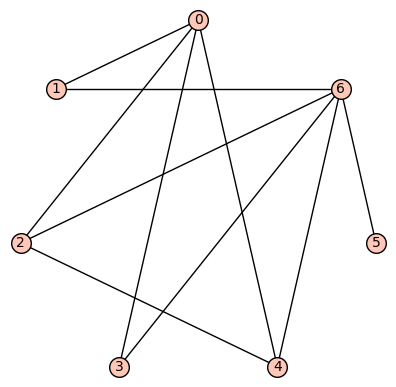
\includegraphics{primer}
\end{align*}

$$radius = 2$$
$$Ra(G) = \frac{1}{\sqrt{4}} + \frac{1}{\sqrt{6}} + \frac{1}{\sqrt{6}} + \frac{1}{\sqrt{6}} + \frac{1}{\sqrt{6}} + \frac{1}{\sqrt{9}} = \frac{5+4\sqrt{6}}{6} \doteq 2.47$$

\vspace{0.5cm}
Vidimo, da na tem grafu lema drži, saj je $2.47 > 2 - 1$.

\pagebreak
\section{Algoritmi}
Oba algoritma sta dostopna na najinem repozitoriju na GitHubu \\
(https://github.com/ZavbiA/Graffiti-conjecture-on-Randic-index-vs.-radius).\\
Algoritem za male grafe se nahaja pod imenom $mali\_grafi.ipynb$, genetski algoritem za večje grafe pa pod imenom $genetic\_algorithm.ipynb$.

\subsection{Algoritem za manjše grafe}
Najprej sva definirala funkcijo, ki za graf vrne Randićev indeks po definirani formuli. Funkcija za izračun radiusa grafa je že vgrajena.
\begin{align*}
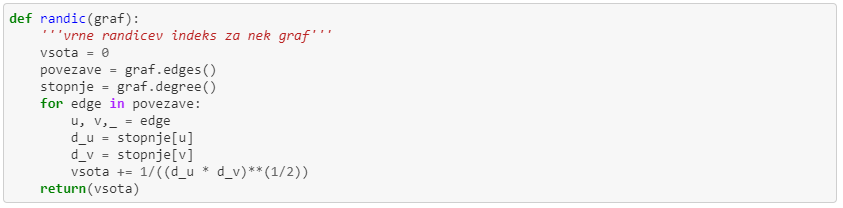
\includegraphics[width=14cm]{randic_mali}
\end{align*}

Nato sva definirala funkcijo, ki za vse grafe velikosti $n$ in manj preveri, ali domneva drži. Tukaj je bila v pomoč funkcija $list(graphs.nauty\_geng(str(i)+" -c"))$, ki vrne seznam vseh enostavnih povezanih grafov velikosti $n$.
\begin{align*}
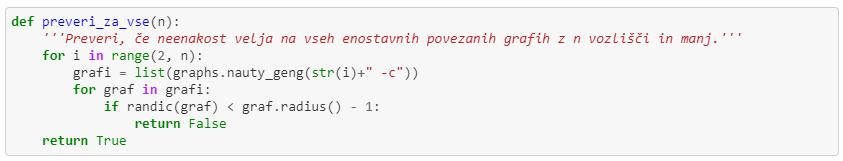
\includegraphics[width=14cm]{preverizavse_mali}
\end{align*}

V kolikor lema za kakšen graf ne bi držala, bi funkcija vrnila $False$, vendar pa se to v nobenem primeru ni zgodilo.
Ta funkcija deluje za grafe do števila vozlišč $n \leq 9$.
Ker je tak algoritem zelo potraten, sva se odločila za uporabo genetskega algoritma.

\subsection{Algoritem za večje grafe}
\

Genetski algoritem je metoda populacijske metahevristike in spada v razdred razvojnih algoritmov. Temelji na ideji evolucije in naravne selekcije, uporablja pa se za generiranje rešitev v optimizaciji s križanjem, mutacijami ipd.

Sestavila sva genetskim algoritmom, s katerim sva poskušala ovreči domnevo.
Ponovno sva najprej definirala Randićev indeks, enako kot pri majhnih grafih.

Nato sva definirala funkcijo $fitness$, ki vrne vrednost neenakosti, torej $Ra(G)-rad(G)+1$. Če bi vrnila negativno vrednost, bi bila lema ovržena.
\begin{align*}
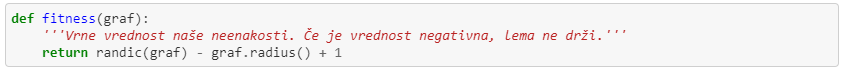
\includegraphics[width=14cm]{fitness}
\end{align*}

Funkcija $fitness\_populacije$ naredi seznam naborov oblike $(graf, njegov fitness)$. Koristna je za hitrejše delovanje algoritma, saj za grafe, za katere je bil $fitness$ že izračunan, le tega ne rabi ponovno računati.
\begin{align*}
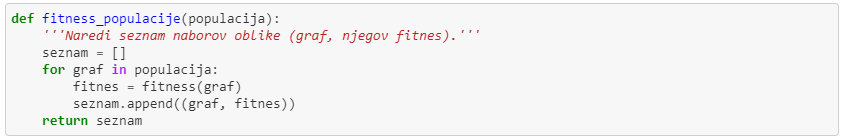
\includegraphics[width=14cm]{fitness_populacije}
\end{align*}

Naslednja funkcija $tournament\_selection$  med t naključno izbranimi grafi izbere tistega, ki ima najmanjšo vrednost funkcije $fitness$. Najprej naključno izbere enega izmed grafov in ga spravi v `najbolsi', nato pa pregleduje ostale grafe in če najde boljšega, ga zamenja. Ravno tako hkrati v $fitnes\_najbolsi$ spravi njegov $fitness$.
(Populacija je že urejena v seznam naborov oblike $(graf, njegov fitness)$.)
\begin{align*}
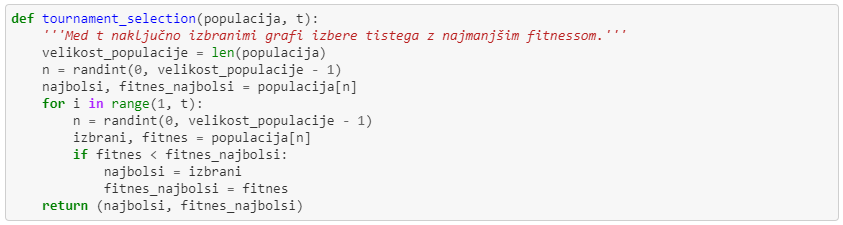
\includegraphics[width=14cm]{tournament_selection}
\end{align*}

Definirala sva funkcijo za Poissonovo porazdelitev, ki pride v poštev kasneje. Z njo bova izbirala število povezav, ki jih bova funkciji $mutiraj$ odstranila oziroma dodala. V funkciji $crossover$ nama pove, koliko povezav bova dodala potomcu.
\begin{align*}
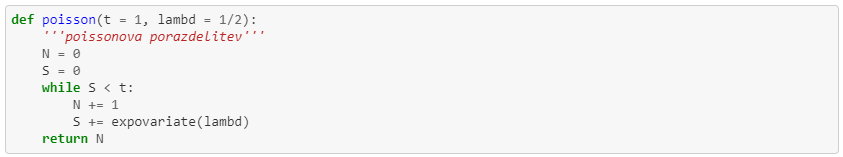
\includegraphics[width=14cm]{poisson}
\end{align*}

Funkcija $mutiraj$ prejme graf in ga mutira. To naredi tako, da najprej naredi kopijo grafa in naključno izbere neko verjetnost. Če je ta verjetnost $\leq\frac{1}{3}$, doda povezavo, če je  $> \frac{1}{3}$ in $\leq \frac{2}{3}$, odstrani povezavo in če je $> \frac{2}{3}$, doda in odstrani povezavo. Ko odstranjujemo povezave, moramo biti pozorni, da graf ostane povezan. V kolikor ni več povezan, je potrebno povezavo dodati nazaj. $Poissonovo$ funkcijo sva uporabila za določitev maksimalnega števila povezav, ki jih grafu lahko dodamo ali odstranimo.
\begin{align*}
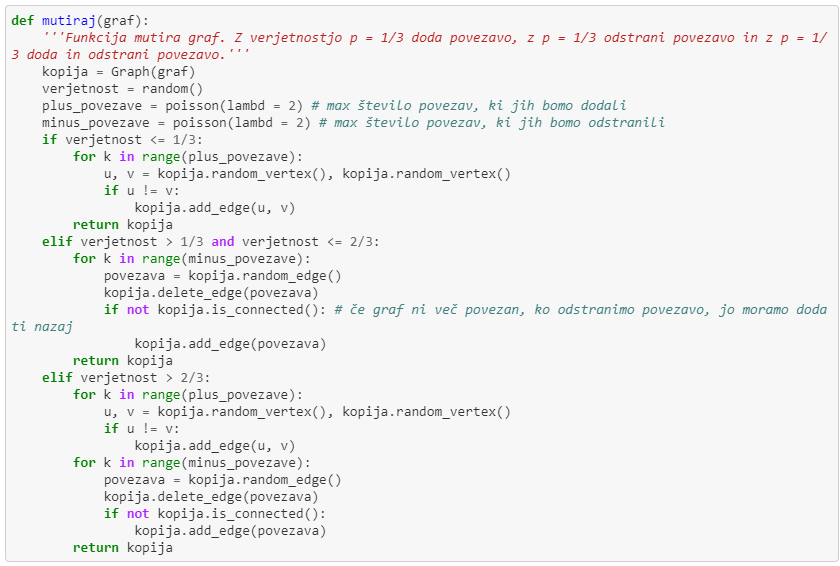
\includegraphics[width=14cm]{mutiraj}
\end{align*}

Funkcija $crossover$ prejme dva grafa ($a$ in $b$) in ju križa med seboj ter vrne njunega potomca. Najprej naredi podgraf grafa $a$, kjer je vsako vozlišče vsebovano z verjetnostjo $\frac{1}{2}$ in prav tako naredi podgraf grafa $b$. Sledi pogoj, da sta oba grafa povezana, imata skupaj $n$ vozlišč in da noben od njiju ni prazen. V $potomec$ najprej shrani povezave, ki med grafoma niso skupne in v $nove\_povezave$ shrani nove povezave, število katerih se seveda veča s številom $n$. Nove povezave naredi s pomočjo $Poissonove$ funkcije. Nato z njimi oblikuje $potomca$. Vmes sva uporabila vgrajeno funkcijo $.relabel()$, ki poskrbi za primerno oštevilčenje vozlišč v novem grafu.
\begin{align*}
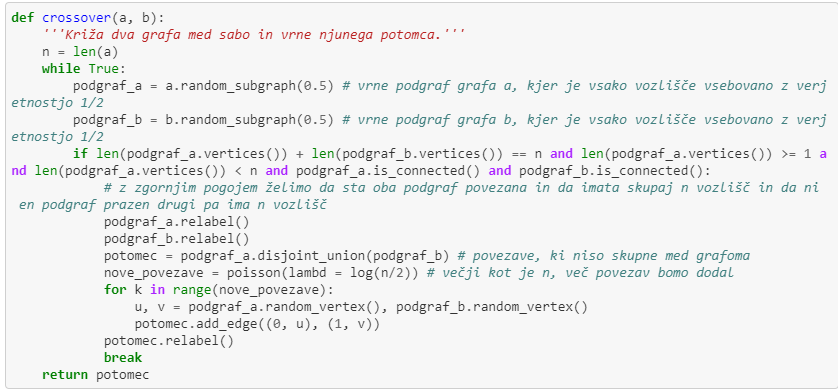
\includegraphics[width=14cm]{crossover}
\end{align*}

Funkcija $zacetna\_populacija$ je potrebna zato, da se naredi začetno populacijo (seznam grafov), kjer imajo grafi $n$ vozlišč. S parametrom $velikost$ je določena velikost populacije, s parametrom $n$ pa število vozlišč grafa. Vsaka povezava v grafu je z neko naključno verjetnostjo. Funkcija poskrbi tudi, da so vsi grafi povezani.
\begin{align*}
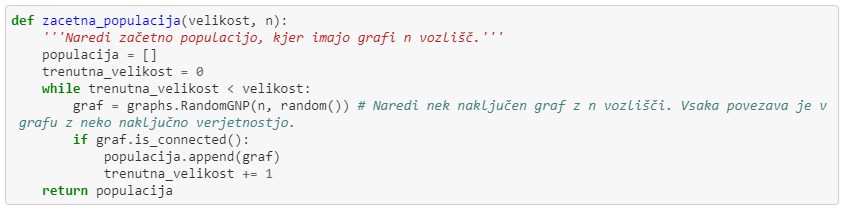
\includegraphics[width=14cm]{zacetna_populacija}
\end{align*}

Funkcija $min\_fitness$ prejme seznam grafov, med katerimi poišče tistega, ki ima najmanjšo vrednost funkcije $fitness$. To pa zato, ker manjša kot je ta vrednost, večja je verjetnost, da bo lema ovržena. Želiva namreč priti pod vrednost 0, večje vrednosti pa lemo le potrdijo za en določen graf. Poleg grafa funkcija vrne tudi njegov $fitness$.
\begin{align*}
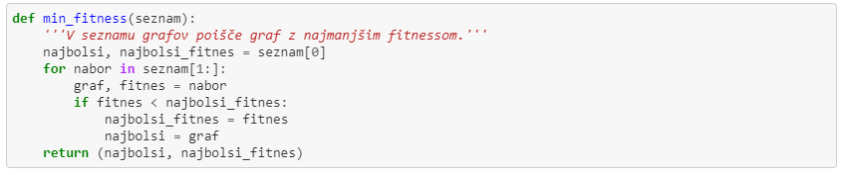
\includegraphics[width=14cm]{min_fitness}
\end{align*}

S funkcijo $nova\_populacija$ iz obstoječe populacije narediva novo populacijo. To narediva z $while$ zanko z mutacijami in križanjem. Funkcija je že tako napisana, da takoj naredi seznam naborov.
\begin{align*}
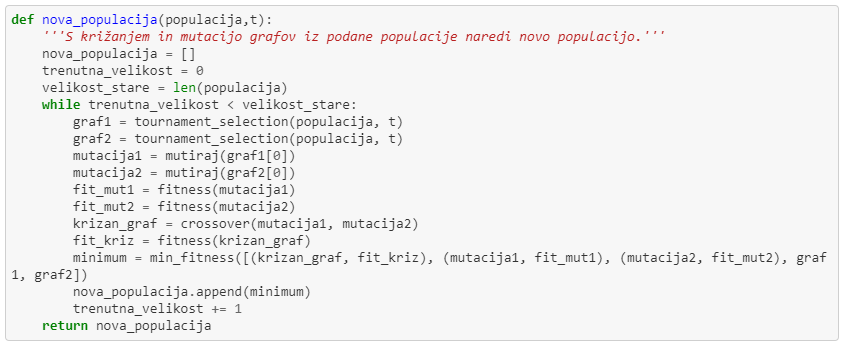
\includegraphics[width=14cm]{nova_populacija}
\end{align*}

Še zadnja funkcija $genetic\_algorithm$ v vsaki ponovitvi s križanjem in mutiranjem naredi novo populacijo. Če v tej populaciji najde graf, za katerega je vrednost $fitness$ manjša od nič, vrne `Lema ne drži' in pripadajoči graf. Če se to ne zgodi pri nobenem grafu, vrne `Ne najdem protiprimera'. Argument $cas\_izvajanja$ je podan zato, da program ne teče v neskončnost. $n$ je velikost populacije (število grafov), $k$ pa je število vozlišč vsakega grafa.
\begin{align*}
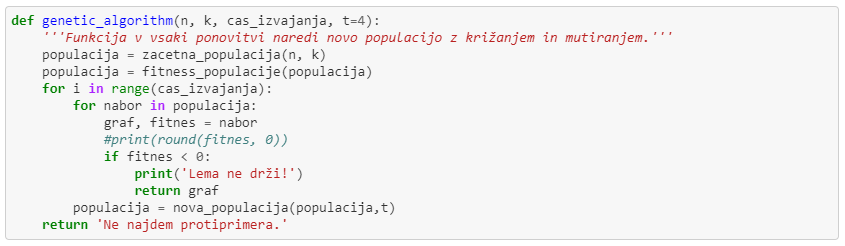
\includegraphics[width=14cm]{genetic_algorithm}
\end{align*}

Lemo sva nato testirala z vnašanjem različnih vrednosti v zadnjo funkcijo in ob tem spremljala časovno zahtevnost.

\section{Ugotovitve}
\subsection{Splošne ugotovitve}
Ugotovila sva, da imajo polni grafi z več kot enim vozliščem radius vedno enak 1. Iz tega dokaj očitno sledi, da neenakost velja (celo stroga neenakost).
Z algoritmom za male grafe sva uspela dokazati, da neenakost drži za vse enostavne povezane grafe s številom vozlišč  $n \leq 9$.
Tudi z genetskim algoritmom za večje grafe pa nama ni uspelo najti protiprimera. Morda bi uspelo s kakšnimi drugimi vhodnimi podatki.
Na podlagi tega leme ne moreva ovreči ali potrditi v celoti.

\subsection{Časovna zahtevnost}
Na čas izvajanja najbolj vpliva velikost grafov. Velikost populacije nima tako velikega vpliva. Populacije morajo biti čim večje, sicer so grafi lahko isti (npr.pri 10 so skoraj gotovo sami isti grafi). S povečevanjem števila ponovitev se linearno veča tudi čas izvajanja.

Z večkratnimi poskusi sva prišla do ugotovitve, da je časovna zahtevnost najinega algoritma enaka $O(čas\_izvajanja * velikost\_populacije * n^2)$.  Čas izvajanja se torej najbolj poveča, če povečava število vozlišč. To pa zato, ker ima funkcija $randic$ casovno zahtevnost $O(n^2)$ in posledično ima isto časovno zahtevnost tudi funkcij $fitness$.  Ker je v funkciji $nova\_populacija$ potrebno za vsak graf izračunati nov $fitness$, je časovna zahtevnost te funkcije enaka $O(velikost\_populacije * n^2)$. V genetskem algoritmu je sicer odvisno, koliko časa se izvaja, ampak  je potrebno v vsaki ponovitvi narediti novo populacijo, zato ima v najinem primeru algoritem časovno zahtevnost $O(čas\_izvajanja * velikost\_populacije * n^2)$.

\pagebreak

\section{Literatura}
\vspace{0.5cm}

\renewcommand{\labelenumi}{[\arabic{enumi}]}
\begin{enumerate}
\item \noindent M. Cygan, M. Pilipczuk, R. Škrekovski, \textsl{On the Inequality between Radius and Randic Index for Graphs}, MATCH, 2011. 
\vspace{0.5cm}
\item \noindent  S. Luke, \textsl{Essentials of Metaheuristics}, Department of Computer Science, George Mason University, Online Version 2.2, 2015.
\end{enumerate}

\end{document}
